\section{Task I : Predicting the Medal of the 2028 LA Olympics}
\subsection{Model Establishment}
Since we want to predict future medal list on the basis of past data, we merge the given data and do some preprocessing. 
We combine the data with the same \textbf{Year} and \textbf{NOC} together.

We use \textbf{Correlation Coefficient Matrix} and \textbf{Principal Component Analysis}, split the data
into training and testing parts, and use \textbf{eXtreme Gradient Boosting} method to train features
and target matrix.

We also use \textbf{KS test} to ensure the effectiveness of the model.After the model is established, we use it to predict the 2028 and 2032 Olympics.

What's important is that we add the factor of whether being a host city/country or not in to the training model so that the final result can take this factor into consideration. For example,
in the coming LA Olympics, the USA is likely to gain more medals due to the \textbf{"hosting effect"}.\cite{davis2018impact}

\subsection{Result Analysis}


According to the results graphs following:

Our model is of decent accuracy, and have an acceptable performance on test set.


\begin{figure}[htbp]
    \centering
    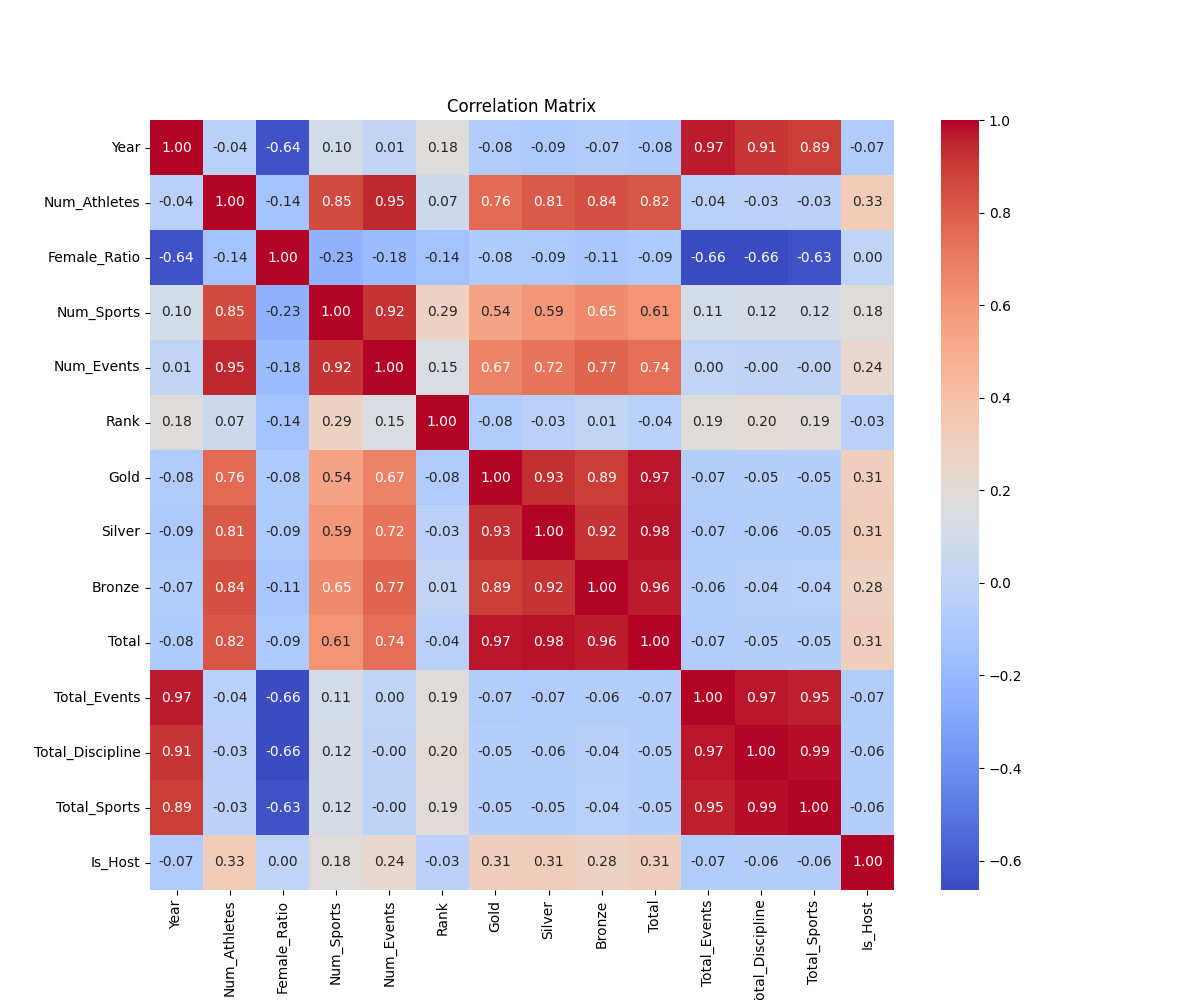
\includegraphics[width=1\textwidth]{./figures/Cor_Matrix.png}
    \caption{Correlation Matrix}
    \label{fig:Cor_Matrix}
\end{figure}

\begin{figure}[htbp]
    \centering
    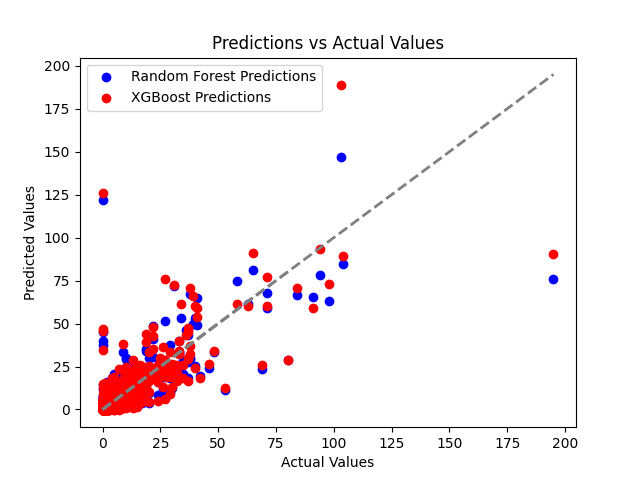
\includegraphics[width=0.8\textwidth]{./figures/K-S_0.png}
    \caption{Method Comparison}
    \label{fig:K-S_0}
\end{figure}

\begin{figure}[htbp]
    \centering
    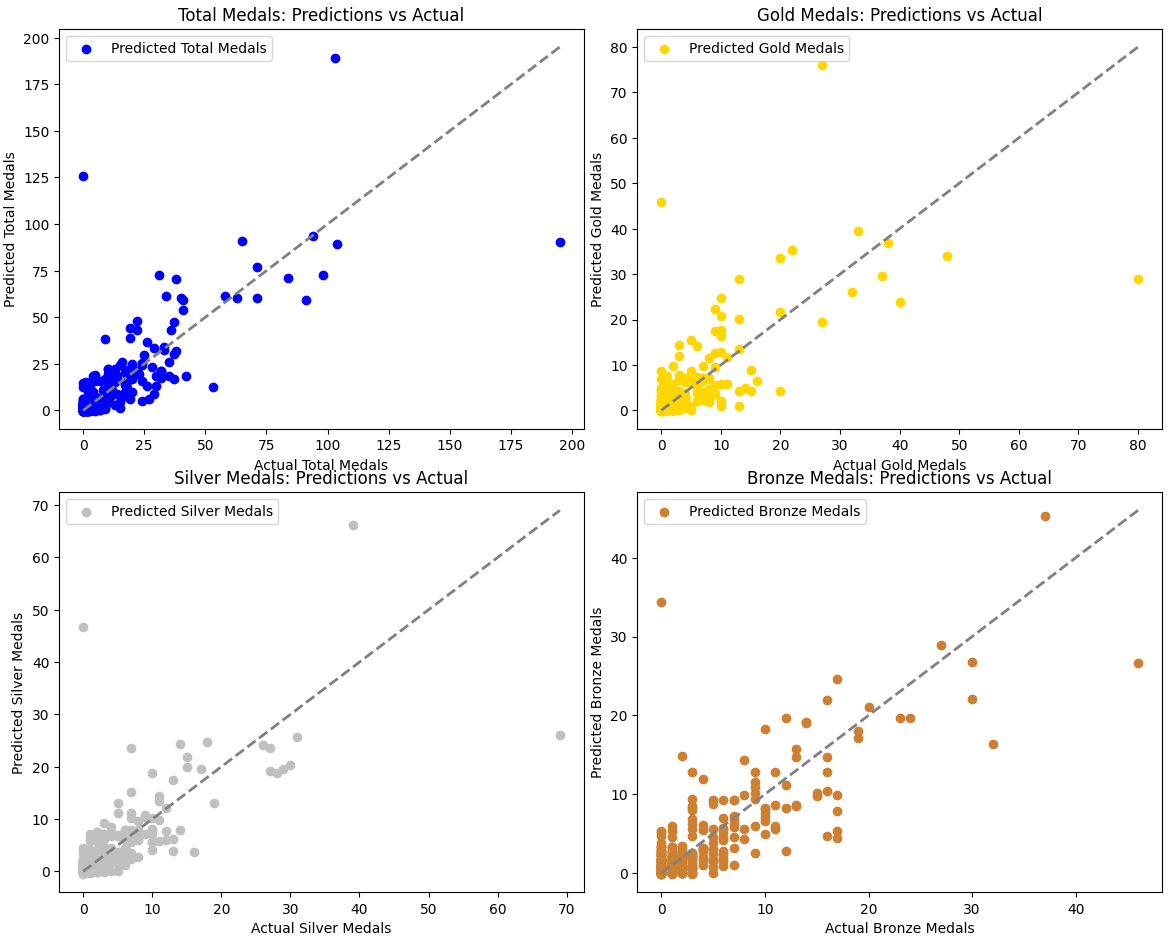
\includegraphics[width=0.8\textwidth]{./figures/K-S_4.png}
    \caption{Precision of the estimation(Gold, Silver, Bronze and Total)}
    \label{fig:K-S_4}
\end{figure}

\begin{figure}[htbp]
    \centering
    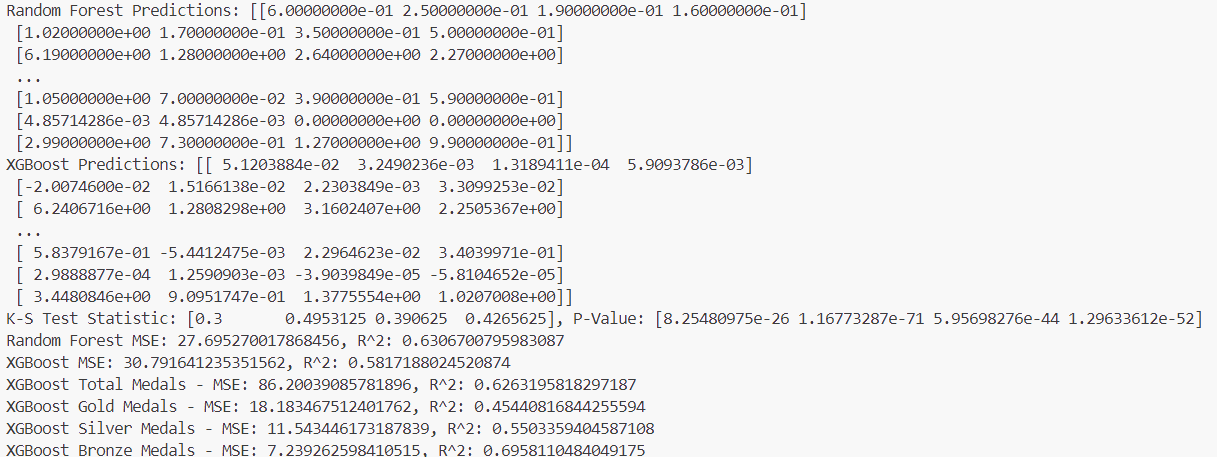
\includegraphics[width=1\textwidth]{./figures/refer_KS_other.png}
    \caption{Measures of Performance}
    \label{fig:refer_KS_other}
\end{figure}

From \textbf{Figure \ref{fig:K-S_0}}, we can see that the prediction of XGBoost outperformed the prediciton of Random Forest Predicitons, which is one of the reason for our choice of model.

As to the specific principle of XGBoost:

\begin{center}
    $\hat{y}_i^{(t)} = \hat{y}_i^{(t-1)} + f_t(x_i)$
\end{center}

The loss function and the objective function are as follows:

$L(\hat{y}_i^{(t-1)}, y_i)$ \quad \text{loss function} $y_i$ \text{prediction from the first to the t-1th tree} $\hat{y}_i^{(t-1)}$

The complete objective function (loss function plus regularization term) can be represented as:
\begin{center}
    $\mathcal{L}^{(t)} = \sum_{i=1}^n L(\hat{y}_i^{(t-1)}, y_i) + \Omega(f_t)$
\end{center}

where $\Omega(f_t)$ is the model complexity of the t-th tree, which can be expressed as:

\begin{center}
    $\Omega(f_t) = \gamma T + \frac{1}{2} \lambda \sum_{j=1}^T w_j^2$
\end{center}

where $T$ is the number of nodes in the tree, $w_j$ is the weight of each node, and $\gamma$ and $\lambda$ are regularization parameters.\cite{smith2023predicting}

\subsection{Prediction of 2028 Los Angeles Olympics}
\begin{table}[htbp]
    \centering
    \caption{Predicted Medal Table of 2028 Los Angeles Olympics with Prediction Intervals}
    \begin{tabular}{|c|c|c|c|c|c|}
        \hline
        Rank & NOC & Gold (Interval) & Silver (Interval) & Bronze (Interval) & Total (Interval) \\
        \hline
        1 & United States & 49 (45, 53) & 46 (42, 50) & 44 (40, 48) & 139 (127, 151) \\
        2 & China & 38 (35, 41) & 30 (27, 33) & 29 (26, 32) & 97 (88, 106) \\
        3 & Russia & 28 (23, 33) & 25 (20, 30) & 22 (17, 27) & 75 (60, 90) \\
        4 & United Kingdom & 27 (25, 29) & 23 (21, 25) & 20 (18, 22) & 70 (64, 76) \\
        5 & Japan & 22 (20, 24) & 19 (17, 21) & 17 (15, 19) & 58 (52, 64) \\
        6 & Australia & 17 (15, 19) & 15 (13, 17) & 13 (11, 15) & 45 (39, 51) \\
        7 & Italy & 15 (13, 17) & 13 (11, 15) & 12 (10, 14) & 40 (34, 46) \\
        8 & Netherlands & 13 (12, 14) & 12 (11, 13) & 11 (10, 12) & 36 (33, 39) \\
        9 & France & 14 (12, 16) & 12 (10, 14) & 9 (7, 11) & 35 (29, 41) \\
        10 & Germany & 15 (13, 17) & 12 (10, 14) & 8 (6, 10) & 35 (29, 41) \\
        \hline
    \end{tabular}
    \label{tab:2028}
\end{table}

As is shown in the table, Ranking may be changed a lot due to the interval of our estimation.

According to our prediction, th United States is likely to win the most medals in the 2028 Los Angeles Olympics, followed by China and Russia. We have assumed that Russia take place in 2028, so it's reasonable for Russia to rank 3rd. Obviously, the United States is most likely to improve its performance in the 2028 Los Angeles Olympics, because it's the host country and they have been performing very well to rank top 1, 2 or 3 for a long time in history.

Russia is a rather special case, since it's performance is almost unpredictable.With the largest interval, it's hard to know whether Russian athletes will improve their performance or not. They have taken too much pressure because of war and doping scandals, which may affect their performance in the future.

Other countries like China, Japan, Germany, Netherlands and so on are very likely to get more medals too. We are not listing all of the countries here, but top 10 countries indicate the main trend.

France is sure to do worse after an excellent performance in the 2024 Paris Olympics, since it's not host country any more. Italy is likely to maintain its performance, while Australia is estimated by our model to do worse although their medal counts are seemingly increasing recent years.